\section{BVR and the Voter Registry}
\label{sec:electorate-size}

The most immediate administrative consequence of biometric registration should appear in the voter registry itself. If the reform improved record quality and eliminated duplicate or outdated registrations, the electorate should contract when municipalities adopt it. If the recadastramento requirement also imposed meaningful compliance costs, that contraction may reflect not only registry cleaning but also temporary or persistent exclusion from the rolls. Those same forces can change the social composition of the electorate, not just its size. For that reason, it is useful to study registry size and registry composition together. In the model, this is the first margin: Proposition~\ref{prop:hetcomp} predicts that once compliance costs are steeper for lower-education citizens, any positive biometric burden should shrink their registration rate more sharply.

This section studies that administrative margin directly. I first describe the event-study specification used for the registry outcomes. I then show that strict BVR produces an immediate contraction in the log number of registered voters. Next, I examine the education margin using both education-specific log counts and education shares, because those two objects distinguish the size of the affected registry groups from the composition of the surviving electorate. I then ask whether the effect is larger in municipalities with weaker pre-treatment connectivity, a descriptive test of the compliance-cost interpretation. The section closes by summarizing the main robustness exercises that support the registry results.

\subsection{Specification and Outcomes}
\label{ssec:bvr-registry-specification}

The registry analysis follows the design in Section~\ref{sec:empirical-design}: a municipality-election panel from 2000 through 2018, strict-BVR treatment timing with ever-hybrid municipalities excluded, never-treated controls, and municipality-clustered standard errors. The figures in this section report the BJS imputation event studies described in Section~\ref{sec:empirical-design} \citep{Borusyak2024RevisitiEventStudy}: pre-period coefficients come from the first-step OLS on untreated cells with leads added as regressors, and post-period coefficients are averages of unit-time effects $\hat{\tau}_{mt} = Y_{mt} - \widehat{Y}_{mt}(0)$ obtained from imputation. Appendix~\hyperref[app:alternative-estimators]{Section~\ref*{app:alternative-estimators}} reports Callaway-Sant'Anna, dynamic TWFE, and de Chaisemartin-D'Haultfoeuille comparisons for the same outcomes; the qualitative pattern is the same across estimators. Event times run from $-8$ to $+8$ in two-year election-cycle steps, with event time $-2$ as the reference period.

The outcomes are chosen to separate three registry objects. The first is the log number of registered voters, which measures the aggregate size of the electorate. The second set is the log number of low- and high-education registrants, which shows how the count of each education group changes around adoption. The third set is the share of the total registered electorate in each education group. These shares are defined over the full electorate, including registrants with missing or unknown schooling, so the low- and high-education shares need not sum mechanically to one.

\subsection{Effect on Electorate Size}
\label{ssec:bvr-electorate-size}

Figure~\ref{fig:bvr-electorate-size} shows the BJS imputation event study for the effect of strict biometric registration on the log number of registered voters. The pattern is sharp. At event time zero, the registry falls by about 0.117 log points, or roughly 11 percent, relative to two years before adoption. The decline then narrows steadily: it is still substantial after one election cycle, but much smaller by six years after adoption, and close to zero by the longest horizon. This sequence is consistent with an immediate wave of removals at the time of recadastramento, followed by gradual re-entry into the registry over subsequent elections. Pre-treatment coefficients are generally small over the immediate pre-period, which is reassuring, although the longest pre- and post-treatment horizons should be interpreted more cautiously because they are identified from the earliest cohorts only.

\begin{figure}[htbp]
    \caption{Biometric Registration and Electorate Size}
    \label{fig:bvr-electorate-size}
    \centering
    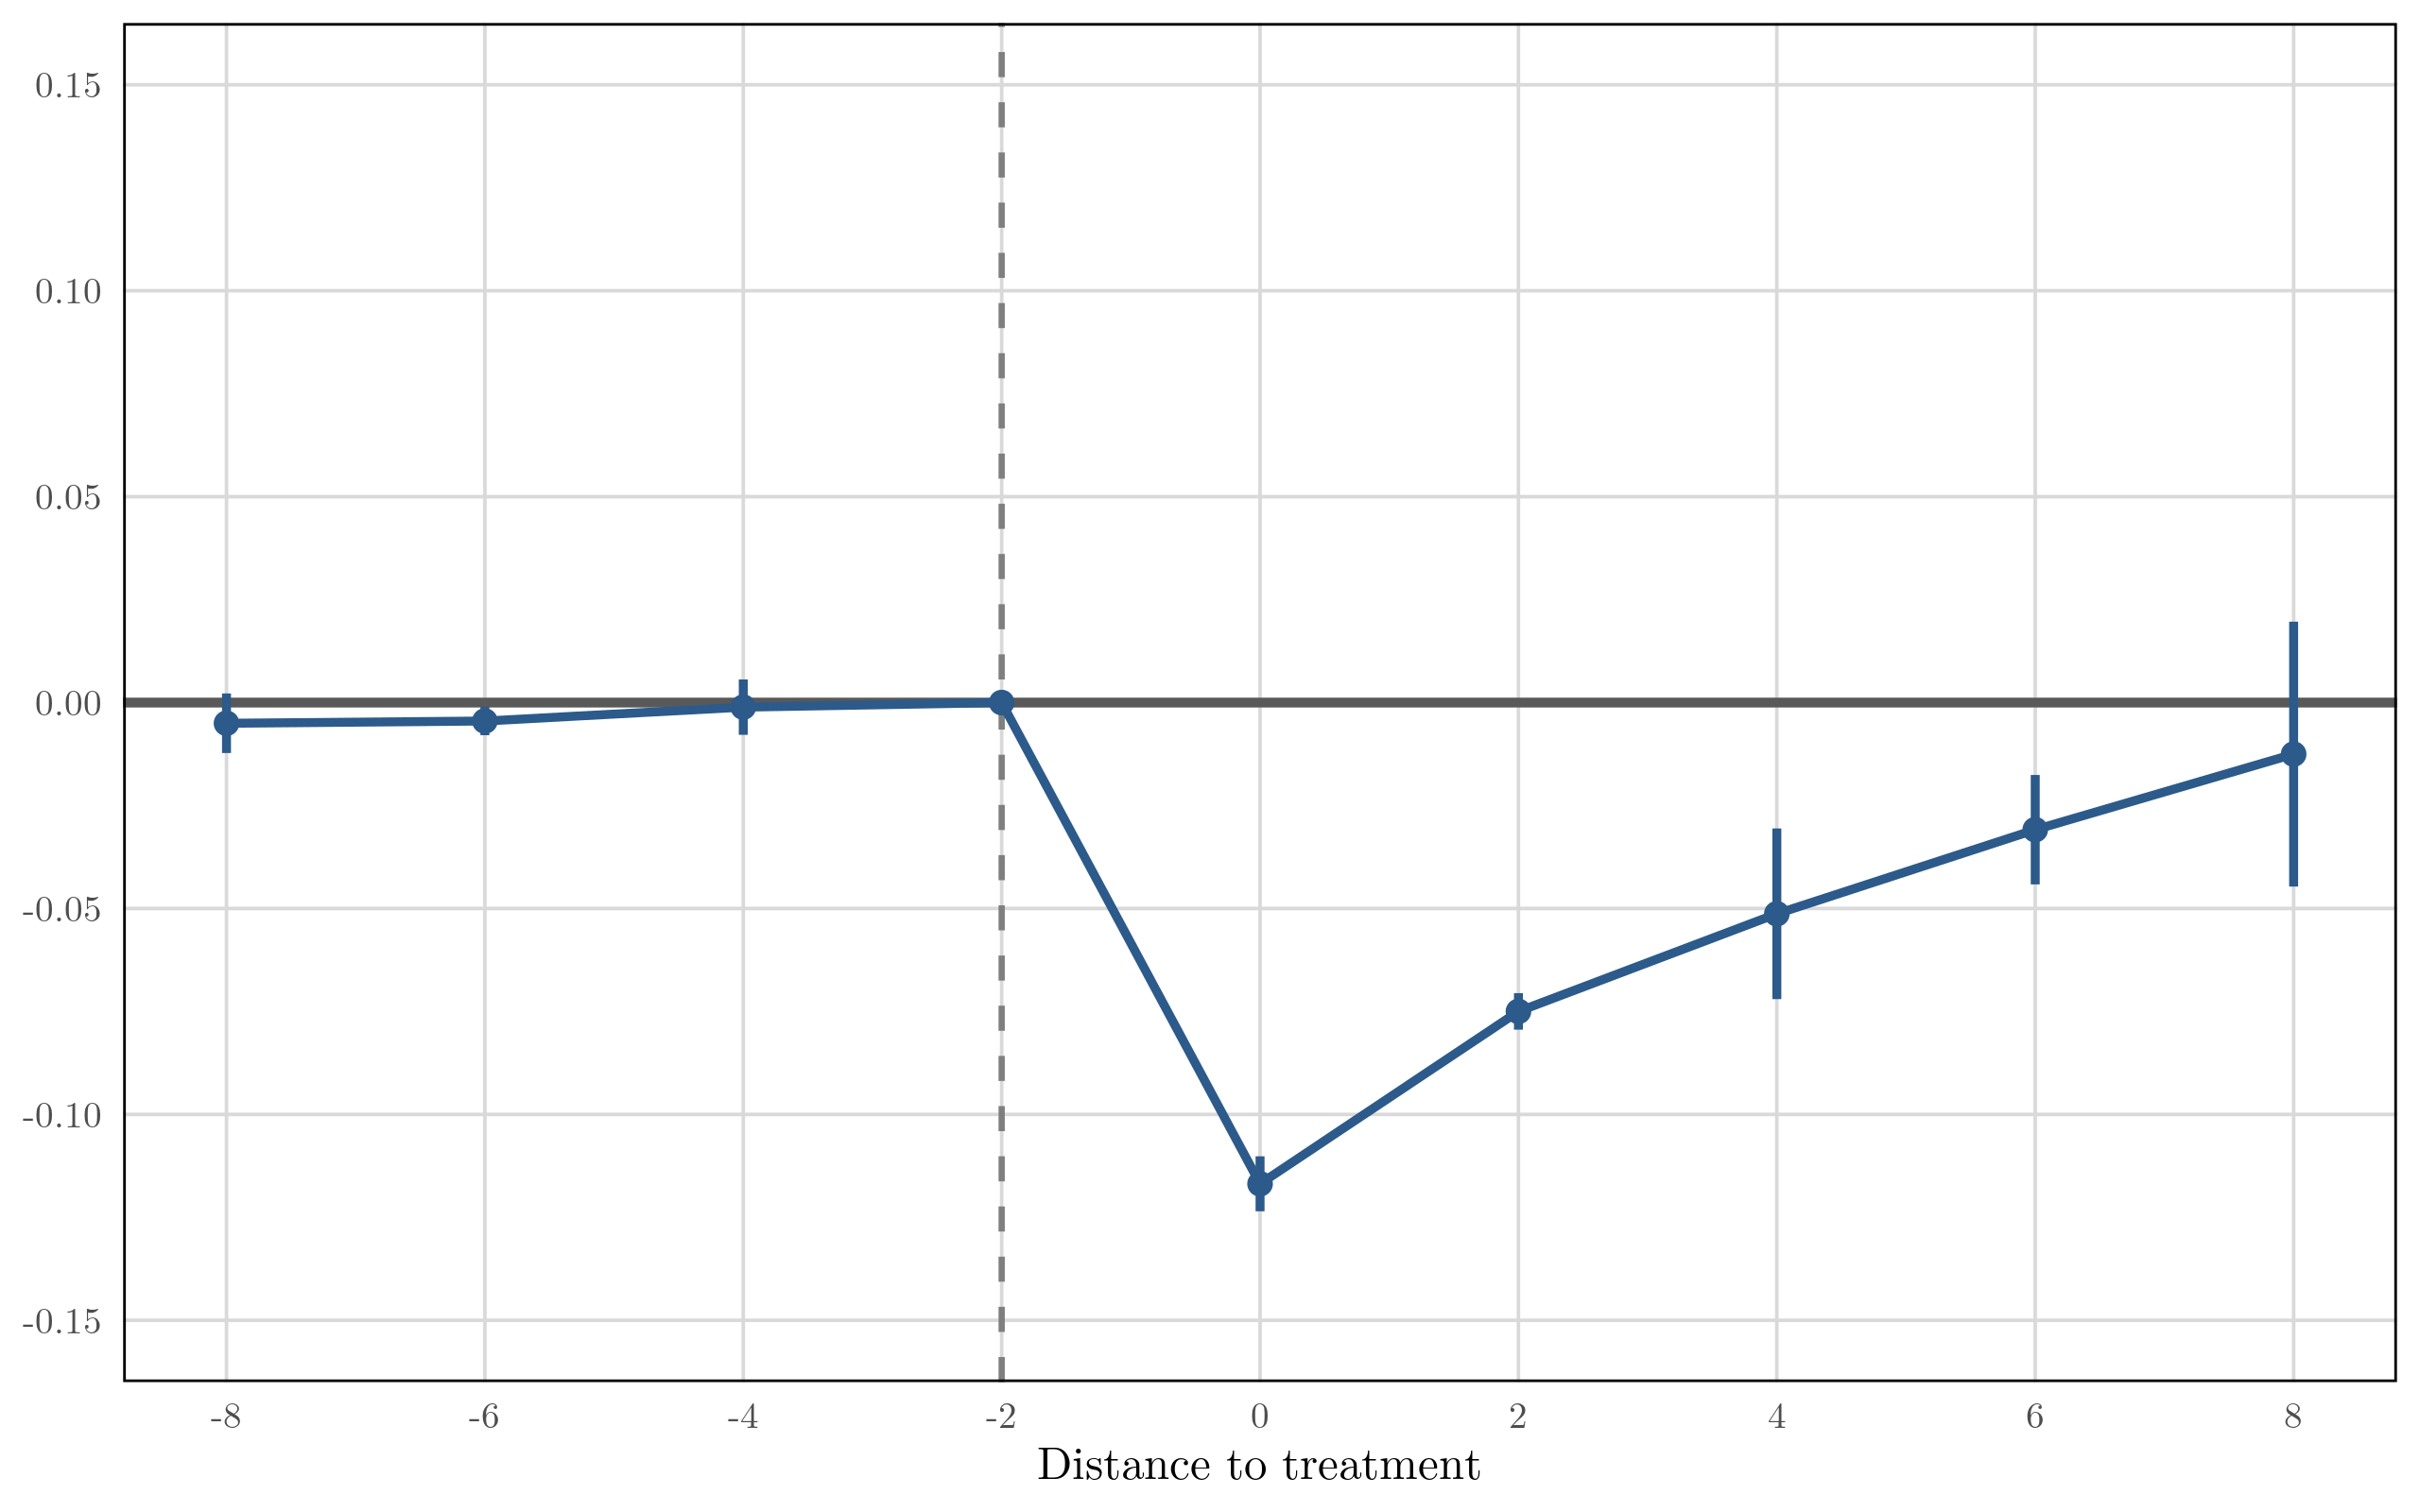
\includegraphics[width=0.72\textwidth]{../resources/regressions/bvr/log_num_voters/strict_bvr/callaway_santanna/event_study_plot.png}
    \vspace{0.75em}
    \begin{minipage}{\textwidth}
        {\footnotesize \textbf{Note:} The figure plots BJS imputation event-study estimates for the log number of registered voters \citep{Borusyak2024RevisitiEventStudy}, using strict BVR municipalities as the treated sample and never-treated municipalities as the control group. Pre-period coefficients are OLS estimates from the first-step regression on untreated cells; post-period coefficients aggregate imputed unit-time effects by event time. Event time $-2$ is the reference period and is shown at zero. Error bars report 95\% confidence intervals with standard errors clustered by municipality. Appendix \hyperref[fig:appendix-size-estimator-comparison]{Figure~\ref*{fig:appendix-size-estimator-comparison}} compares the same outcome across alternative staggered-adoption estimators. \par}
    \end{minipage}
\end{figure}

\subsection{Effects by Education Level}
\label{sec:electorate-composition}
\label{ssec:bvr-education-levels}

Biometric registration did not simply change the number of voters on the rolls; it also changed who remained on them. That distinction matters for political economy because a reform that improves registry integrity but imposes unequal compliance costs can reallocate political voice even if aggregate registration later recovers. The \TSE{} electorate files make it possible to track registered voters by schooling at the municipality-election level. Following the definitions in Section~\ref{sec:data-and-measurement}, I classify low education as all categories below completed secondary schooling and high education as incomplete secondary schooling or more. The Brazilian electorate was already becoming more educated over time: the electorate-weighted share of low-education registrants fell from 72.8\% in 2000 to 63.9\% in 2008 and 46.2\% in 2018, while the corresponding high-education share rose from 27.0\% to 36.0\% and 53.8\%. Those aggregate trends make simple cross-sectional comparisons uninformative. The relevant question is whether municipalities change discontinuously around biometric adoption relative to comparable municipalities that have not yet adopted the reform. That compositional margin is also what drives Proposition~\ref{prop:drift_sign}: if the surviving electorate becomes relatively more educated, the downstream equilibrium policy should tilt away from redistribution even when the aggregate registry later recovers.

Figure~\ref{fig:bvr-education-counts} reports the education-specific log-count event studies. The low-education registry contracts sharply at adoption, falling by about 0.254 log points at event time zero. By contrast, the high-education count rises by about 0.149 log points at the same horizon. The two series therefore show that the aggregate registry contraction is concentrated among low-education records and is accompanied by an increase in high-education records. That pattern is consistent with differential compliance costs, but it also points to the possibility of education-record updating during recadastramento, a mechanism that the decomposition section investigates more directly.

\begin{figure}[htbp]
    \caption{Biometric Registration and Education-Specific Registry Counts}
    \label{fig:bvr-education-counts}
    \centering
    \begin{subfigure}[b]{0.49\textwidth}
        \centering
        
\includegraphics[width=\textwidth]{../resources/regressions/bvr/log_num_voters_low_ed/strict_bvr/callaway_santanna/event_study_plot.png}
        \caption{Low-education registrants}
        \label{fig:bvr-low-education-log-counts}
    \end{subfigure}
    \hfill
    \begin{subfigure}[b]{0.49\textwidth}
        \centering
        
\includegraphics[width=\textwidth]{../resources/regressions/bvr/log_num_voters_high_ed/strict_bvr/callaway_santanna/event_study_plot.png}
        \caption{High-education registrants}
        \label{fig:bvr-high-education-log-counts}
    \end{subfigure}
    \vspace{0.75em}
    \begin{minipage}{\textwidth}
        {\footnotesize \textbf{Note:} Each panel plots BJS imputation event-study estimates for log education-specific registered-voter counts \citep{Borusyak2024RevisitiEventStudy}, using strict BVR municipalities as the treated sample and never-treated municipalities as the control group. Pre-period coefficients are OLS estimates from the first-step regression on untreated cells; post-period coefficients aggregate imputed unit-time effects by event time. Municipalities ever coded as hybrid are excluded. Event time $-2$ is the reference period and is shown at zero. Error bars report 95\% confidence intervals with standard errors clustered by municipality. Both panels use the same y-axis range and tick marks. \par}
    \end{minipage}
\end{figure}

Figure~\ref{fig:bvr-education-composition} reports the corresponding BJS imputation event-study estimates for the low- and high-education shares. The effects are large on impact. At event time zero, biometric registration lowers the low-education share by 8.9 percentage points and raises the high-education share by 9.0 percentage points. The estimates then partially unwind as the registry recovers, but they do not disappear. Eight years after adoption, the low-education share remains 5.9 percentage points below its pre-treatment level, while the high-education share remains 5.9 points above it. Because these education shares are defined over the total electorate, including voters with missing schooling, they need not mechanically sum to one. The near mirror-image responses therefore point to a genuine reweighting of the registered electorate toward more educated voters rather than a purely mechanical denominator effect.

\begin{figure}[htbp]
    \caption{Biometric Registration and Education Composition}
    \label{fig:bvr-education-composition}
    \centering
    \begin{subfigure}[b]{0.49\textwidth}
        \centering
        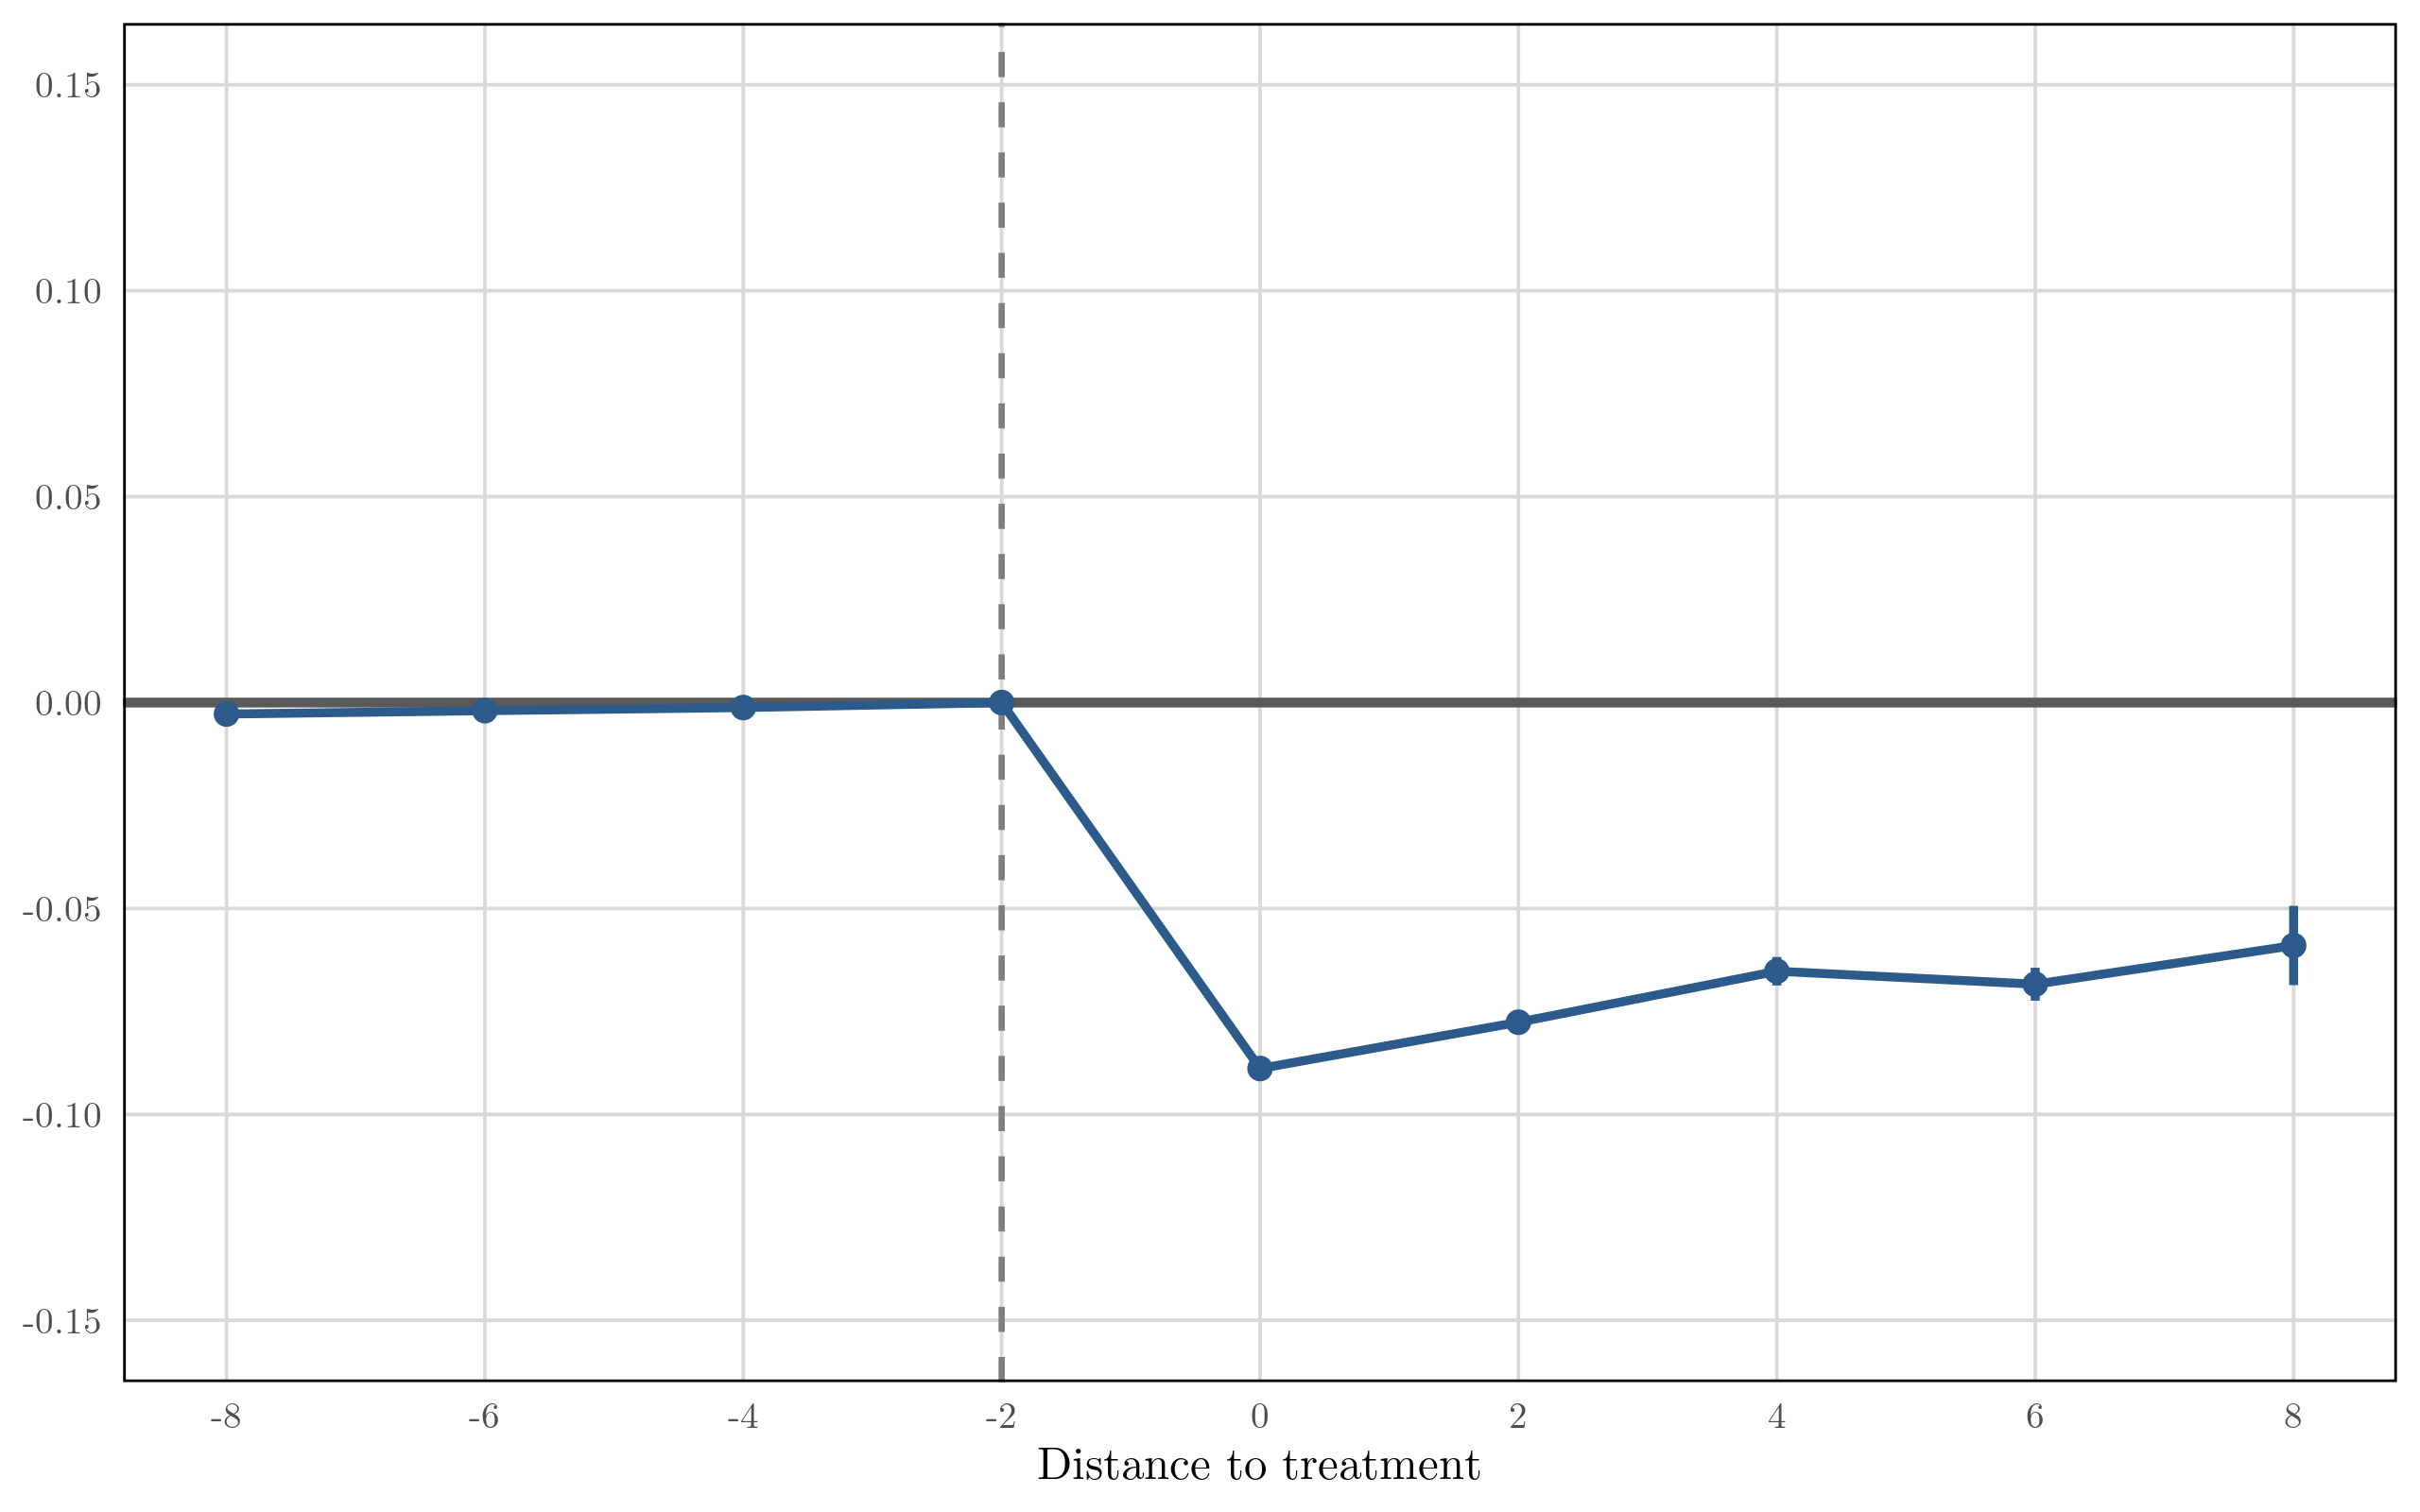
\includegraphics[width=\textwidth]{../resources/regressions/bvr/pct_voters_low_ed/strict_bvr/callaway_santanna/event_study_plot.png}
        \caption{Low-education share}
        \label{fig:bvr-low-education-share}
    \end{subfigure}
    \hfill
    \begin{subfigure}[b]{0.49\textwidth}
        \centering
        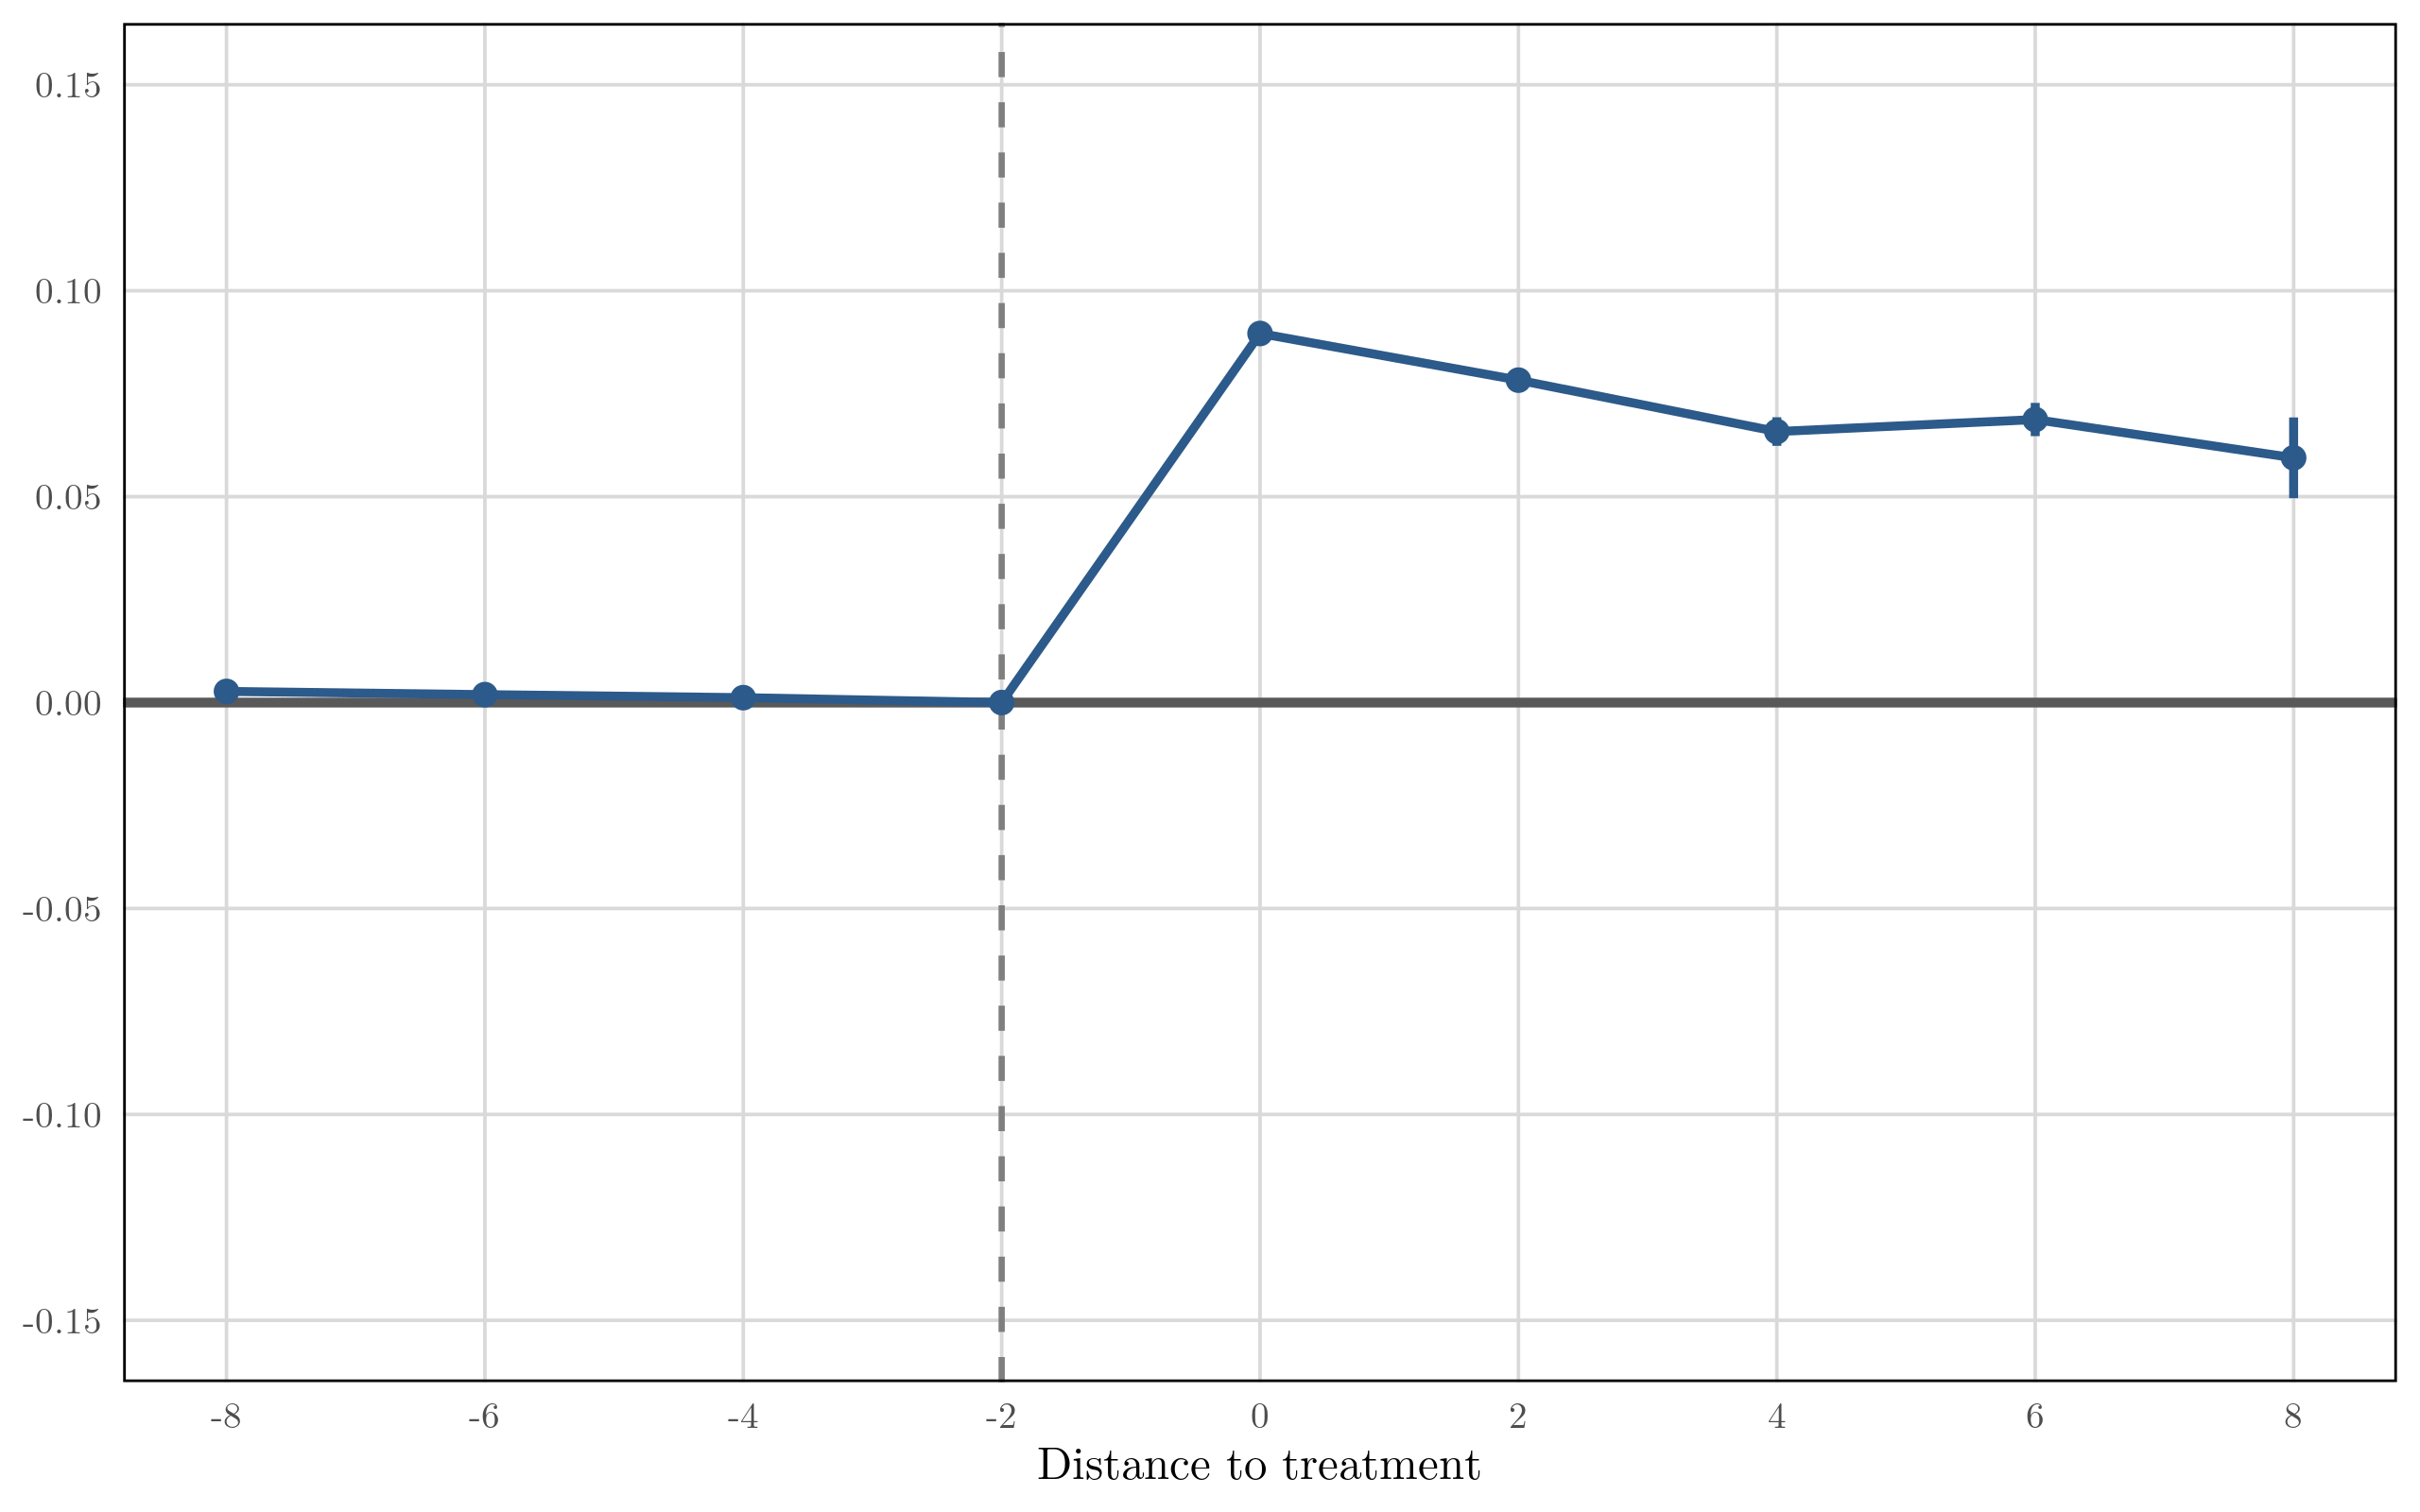
\includegraphics[width=\textwidth]{../resources/regressions/bvr/pct_voters_high_ed/strict_bvr/callaway_santanna/event_study_plot.png}
        \caption{High-education share}
        \label{fig:bvr-high-education-share}
    \end{subfigure}
    \vspace{0.75em}
    \begin{minipage}{\textwidth}
        {\footnotesize \textbf{Note:} Each panel plots BJS imputation event-study estimates \citep{Borusyak2024RevisitiEventStudy}, using strict BVR municipalities as the treated sample and never-treated municipalities as the control group. Pre-period coefficients are OLS estimates from the first-step regression on untreated cells; post-period coefficients aggregate imputed unit-time effects by event time. Event time $-2$ is the reference period and is shown at zero. Error bars report 95\% confidence intervals with standard errors clustered by municipality. Panel (a) uses the share of registered voters with schooling below completed secondary education as the outcome. Panel (b) uses the share with incomplete secondary schooling or more. Appendix \hyperref[fig:appendix-composition-estimator-comparison]{Figure~\ref*{fig:appendix-composition-estimator-comparison}} reports the corresponding comparison figures for alternative staggered-adoption estimators. \par}
    \end{minipage}
\end{figure}

One plausible channel is differential compliance: the in-person recadastramento requirement may have imposed larger administrative burdens on lower-education voters, leading to more cancellations or slower re-entry in those groups. A second channel is information updating. Re-registration may have improved the quality of education records, so some of the persistent shift could reflect cleaner measurement rather than exclusion alone. Taken together with the earlier evidence on registry size, the most credible interpretation is that biometric registration both cleaned the rolls and changed their composition.

\subsection{Effects by Connectivity}
\label{ssec:connectivity-heterogeneity}

The main registry result raises a natural mechanism question: did the same biometric requirement impose different compliance costs across municipalities with different information infrastructure? Biometric recadastramento required citizens to learn about the revision process, appear before the electoral bureaucracy, and update administrative records before the next election. Those requirements are likely to be less costly in places where citizens and local organizations can more easily receive information, coordinate appointments, or monitor administrative deadlines. This is the same logic that motivates the literature on registration costs and administrative burdens: procedural rules need not be facially discriminatory to have unequal participation effects when the cost of compliance is unevenly distributed \citep{Rosenstone1978TheEffectRegistra, Ansolabehere2005TheIntroducVoter, Herd2018}.

To examine this possibility, I split municipalities by pre-treatment connectivity. I use fixed broadband density in 2008, before the main expansion of biometric registration, and compare municipalities in the bottom third of the distribution to municipalities in the top third. I leave the middle third out of the figure so that the comparison is between municipalities with clearly different pre-existing communication infrastructure. This split should be read as heterogeneity in exposure to an administrative environment, not as a causal estimate of the effect of broadband access itself. It is useful because the theory predicts that BVR should contract the registry most where compliance costs are high, but the exercise is descriptive because connectivity is bundled with many other municipal characteristics.

Figure~\ref{fig:bvr-connectivity-heterogeneity} reports the dynamic registry effects separately for low- and high-connectivity municipalities. The specification mirrors the baseline BJS imputation event study for electorate size: strict BVR is the treatment, municipalities ever coded as hybrid are excluded, never-treated municipalities form the control group, event time $-2$ is the reference period, and standard errors are clustered by municipality. The axes are held fixed across the two panels so that the magnitudes can be compared visually.

\begin{figure}[htbp]
    \caption{Biometric Registration and Electorate Size by Pre-BVR Connectivity}
    \label{fig:bvr-connectivity-heterogeneity}
    \centering
    \begin{subfigure}[b]{0.49\textwidth}
        \centering
        \includegraphics[width=\textwidth]{../resources/figures/bvr_connectivity/callaway_style/cs_log_num_voters_low_connectivity_notitle.pdf}
        \caption{Low connectivity}
        \label{fig:bvr-low-connectivity}
    \end{subfigure}
    \hfill
    \begin{subfigure}[b]{0.49\textwidth}
        \centering
        \includegraphics[width=\textwidth]{../resources/figures/bvr_connectivity/callaway_style/cs_log_num_voters_high_connectivity_notitle.pdf}
        \caption{High connectivity}
        \label{fig:bvr-high-connectivity}
    \end{subfigure}
    \vspace{0.75em}
    \begin{minipage}{\textwidth}
        {\footnotesize \textbf{Note:} Each panel plots dynamic event-study estimates for the log number of registered voters, splitting the strict-BVR sample by 2008 fixed broadband density. Panel (a) keeps municipalities in the bottom third of the 2008 connectivity distribution, and panel (b) keeps municipalities in the top third. The middle third is omitted from the figure. Never-treated municipalities within the corresponding connectivity group are the control group. Event time $-2$ is the reference period and is shown at zero. Error bars report 95\% confidence intervals with standard errors clustered by municipality. Both panels use the same y-axis range and tick marks. \par}
    \end{minipage}
\end{figure}

The pattern is consistent with connectivity moderating the administrative burden of BVR. At adoption, the estimated registry contraction is about 0.136 log points in low-connectivity municipalities and about 0.100 log points in high-connectivity municipalities. The difference persists after adoption. Two election cycles after treatment, the low-connectivity estimate remains close to $-0.092$, while the high-connectivity estimate has narrowed to about $-0.025$. By the longest horizon, the high-connectivity series is essentially back to zero, whereas the low-connectivity series remains around $-0.094$. This contrast suggests that the initial registry cleaning and subsequent re-entry process were more costly, slower, or less complete in places with weaker pre-existing connectivity.

This heterogeneity matters for the paper's interpretation because it links the aggregate registry contraction to a concrete mechanism. The main estimates show that BVR reduced the number of registered voters; the connectivity split suggests that the effect was not only a uniform administrative purge of invalid records. If the reform were only removing obsolete or duplicate registrations with no meaningful compliance burden for valid voters, there would be less reason to expect the contraction to be systematically larger in low-connectivity municipalities. The stronger effect in less connected places is instead consistent with a compliance-cost channel: information frictions, travel burdens, bureaucratic uncertainty, and weaker local administrative support may have made it harder for eligible citizens to complete recadastramento on time.

The result also clarifies how biometric registration differs from earlier electoral technologies in Brazil. Electronic voting reduced ballot error and increased the political weight of less-educated voters by making vote casting easier at the polling place \citep{Fujiwara2015VotingTechnoloPolitica}. Biometric registration is a different kind of modernization. It can improve the credibility and quality of the registry, but it operates before election day and therefore requires citizens to pass through an administrative process in order to remain eligible. In that sense, the relevant state-capacity question is not only whether the technology works, but whether the infrastructure around the technology allows citizens to comply with it. This connects the result to broader evidence that biometric and digital state-capacity investments can improve service delivery while raising distributional concerns about who can access the new administrative interface \citep{Muralidharan2016BuildingStateCapacity, Bossuroy2024BiometriMonitoriService}.

At the same time, the connectivity split has important shortcomings. Low- and high-connectivity municipalities are not otherwise comparable places. Appendix Table~\ref{tab:connectivity-balance} shows that high-connectivity municipalities are larger, richer, much more likely to be in the South and Southeast, and have substantially lower baseline low-education shares. Low-connectivity municipalities are concentrated in the North and Northeast and have lower 2008 GDP per capita. These differences matter because fixed broadband density is a proxy for a broader bundle of municipal development and state capacity, not an isolated source of quasi-random variation. The same factors that predict connectivity may also predict the quality of electoral administration, the availability of registry offices, the intensity of local outreach, and citizens' ability to absorb bureaucratic shocks \citep{besleyPersson2011, AcemogluRobinson2019}.

For this reason, I interpret Figure~\ref{fig:bvr-connectivity-heterogeneity} as mechanism evidence rather than as an independent causal design. The exercise shows that BVR's registry effects are larger where pre-existing communication infrastructure is weaker, which is exactly the direction predicted by a compliance-cost interpretation. It does not prove that broadband access itself protected voters from exclusion. A stronger version of the analysis would residualize connectivity with respect to baseline municipal characteristics, compare municipalities within narrower regional support, or exploit supply-side changes in telecommunications infrastructure. The present result is therefore best viewed as a disciplined descriptive check: it supports the claim that administrative modernization can have unequal consequences across local state-capacity environments, while also making clear that those environments differ along many dimensions.

Finally, the result helps discipline the welfare interpretation developed below. If BVR's costs were borne evenly across space, the main normative question would be the aggregate tradeoff between registry integrity and total registry contraction. The connectivity gradient points to a more distributional problem. Modernization may improve the average quality of electoral administration while imposing its largest participation costs on places least able to navigate the transition. That is why the welfare analysis treats compliance costs as heterogeneous and why the empirical decomposition focuses not only on how many registrants disappear, but also on which citizens and which municipalities are most exposed to the administrative burden.

\subsection{Robustness}
\label{ssec:bvr-registry-robustness}

The appendix reports several complementary checks. First, Appendix \hyperref[app:including-hybrid]{Section~\ref*{app:including-hybrid}} repeats the BJS imputation event studies after including hybrid municipalities in the treatment definition. The resulting estimates have the same signs and dynamic shape but are smaller at impact, consistent with hybrid BVR being a lower-intensity version of the reform. Second, Appendix \hyperref[fig:appendix-size-estimator-comparison]{Figure~\ref*{fig:appendix-size-estimator-comparison}} reports the estimator-comparison exercise for registry size, and Appendix \hyperref[fig:appendix-composition-estimator-comparison]{Figure~\ref*{fig:appendix-composition-estimator-comparison}} does the same for the education shares. Across the BJS imputation baseline and the Callaway-Sant'Anna, dynamic TWFE, and de Chaisemartin-D'Haultfoeuille comparisons, the main qualitative conclusions are stable: the registry contracts at adoption and then recovers, while the electorate shifts away from lower-education registrants and toward higher-education registrants. Third, Appendix \hyperref[app:honestdid]{Section~\ref*{app:honestdid}} applies Rambachan-Roth sensitivity analysis to the event-time $0$ coefficients; under the relative-magnitudes restriction, the breakdown value exceeds $\bar{M}=2$ for all three outcomes, so the impact estimates remain statistically separated from zero even when post-treatment confounding is allowed to be more than twice as large as the worst observed pre-trend deviation. Fourth, Appendix \hyperref[app:additional-robustness]{Section~\ref*{app:additional-robustness}} reports state $\times$ election-year fixed effects, within-state-support restrictions, permutation tests, negative-weight diagnostics, and cohort-balance checks, which together strengthen the case for relying on within-municipality event-time comparisons rather than simple cross-sectional contrasts.
